\documentclass[journal,12pt,twocolumn]{IEEEtran}
%
\usepackage{setspace}
\usepackage{gensymb}
\usepackage{siunitx}
\usepackage{tkz-euclide} 
\usepackage{textcomp}
\usepackage{standalone}
\usetikzlibrary{calc}
\newcommand\hmmax{0}
\newcommand\bmmax{0}

%\doublespacing
\singlespacing

%\usepackage{graphicx}
%\usepackage{amssymb}
%\usepackage{relsize}
\usepackage[cmex10]{amsmath}
%\usepackage{amsthm}
%\interdisplaylinepenalty=2500
%\savesymbol{iint}
%\usepackage{txfonts}
%\restoresymbol{TXF}{iint}
%\usepackage{wasysym}
\usepackage{amsthm}
%\usepackage{iithtlc}
\usepackage{mathrsfs}
\usepackage{txfonts}
\usepackage{stfloats}
\usepackage{bm}
\usepackage{cite}
\usepackage{cases}
\usepackage{subfig}
%\usepackage{xtab}
\usepackage{longtable}
\usepackage{multirow}
%\usepackage{algorithm}
%\usepackage{algpseudocode}
\usepackage{enumitem}
\usepackage{mathtools}
\usepackage{steinmetz}
\usepackage{tikz}
\usepackage{circuitikz}
\usepackage{verbatim}
\usepackage{tfrupee}
\usepackage[breaklinks=true]{hyperref}
%\usepackage{stmaryrd}
\usepackage{tkz-euclide} % loads  TikZ and tkz-base
%\usetkzobj{all}
\usetikzlibrary{calc,math}
\usepackage{listings}
    \usepackage{color}                                            %%
    \usepackage{array}                                            %%
    \usepackage{longtable}                                        %%
    \usepackage{calc}                                             %%
    \usepackage{multirow}                                         %%
    \usepackage{hhline}                                           %%
    \usepackage{ifthen}                                           %%
  %optionally (for landscape tables embedded in another document): %%
    \usepackage{lscape}     
\usepackage{multicol}
\usepackage{chngcntr}
\usepackage{amsmath}
\usepackage{cleveref}
\usepackage{amsmath}
%\usepackage{enumerate}

%\usepackage{wasysym}
%\newcounter{MYtempeqncnt}
\DeclareMathOperator*{\Res}{Res}
%\renewcommand{\baselinestretch}{2}
\renewcommand\thesection{\arabic{section}}
\renewcommand\thesubsection{\thesection.\arabic{subsection}}
\renewcommand\thesubsubsection{\thesubsection.\arabic{subsubsection}}

\renewcommand\thesectiondis{\arabic{section}}
\renewcommand\thesubsectiondis{\thesectiondis.\arabic{subsection}}
\renewcommand\thesubsubsectiondis{\thesubsectiondis.\arabic{subsubsection}}

% correct bad hyphenation here
\hyphenation{op-tical net-works semi-conduc-tor}
\def\inputGnumericTable{}                                 %%

\lstset{
%language=C,
frame=single, 
breaklines=true,
columns=fullflexible
}
%\lstset{
%language=tex,
%frame=single, 
%breaklines=true
%}
\usepackage{graphicx}
\usepackage{pgfplots}

\begin{document}


\newtheorem{theorem}{Theorem}[section]
\newtheorem{problem}{Problem}
\newtheorem{proposition}{Proposition}[section]
\newtheorem{lemma}{Lemma}[section]
\newtheorem{corollary}[theorem]{Corollary}
\newtheorem{example}{Example}[section]
\newtheorem{definition}[problem]{Definition}
%\newtheorem{thm}{Theorem}[section] 
%\newtheorem{defn}[thm]{Definition}
%\newtheorem{algorithm}{Algorithm}[section]
%\newtheorem{cor}{Corollary}
\newcommand{\BEQA}{\begin{eqnarray}}
\newcommand{\EEQA}{\end{eqnarray}}
\newcommand{\define}{\stackrel{\triangle}{=}}
\bibliographystyle{IEEEtran}
%\bibliographystyle{ieeetr}
\providecommand{\mbf}{\mathbf}
\providecommand{\abs}[1]{\ensuremath{\left\vert#1\right\vert}}
\providecommand{\norm}[1]{\ensuremath{\left\lVert#1\right\rVert}}
\providecommand{\mean}[1]{\ensuremath{E\left[ #1 \right]}}
\providecommand{\pr}[1]{\ensuremath{\Pr\left(#1\right)}}
\providecommand{\qfunc}[1]{\ensuremath{Q\left(#1\right)}}
\providecommand{\sbrak}[1]{\ensuremath{{}\left[#1\right]}}
\providecommand{\lsbrak}[1]{\ensuremath{{}\left[#1\right.}}
\providecommand{\rsbrak}[1]{\ensuremath{{}\left.#1\right]}}
\providecommand{\brak}[1]{\ensuremath{\left(#1\right)}}
\providecommand{\lbrak}[1]{\ensuremath{\left(#1\right.}}
\providecommand{\rbrak}[1]{\ensuremath{\left.#1\right)}}
\providecommand{\cbrak}[1]{\ensuremath{\left\{#1\right\}}}
\providecommand{\lcbrak}[1]{\ensuremath{\left\{#1\right.}}
\providecommand{\rcbrak}[1]{\ensuremath{\left.#1\right\}}}
\theoremstyle{remark}
\newtheorem{rem}{Remark}
\newcommand{\sgn}{\mathop{\mathrm{sgn}}}
\providecommand{\res}[1]{\Res\displaylimits_{#1}} 
%\providecommand{\norm}[1]{\lVert#1\rVert}
\providecommand{\mtx}[1]{\mathbf{#1}}
\providecommand{\fourier}{\overset{\mathcal{F}}{ \rightleftharpoons}}
%\providecommand{\hilbert}{\overset{\mathcal{H}}{ \rightleftharpoons}}
\providecommand{\system}{\overset{\mathcal{H}}{ \longleftrightarrow}}
	%\newcommand{\solution}[2]{\textbf{Solution:}{#1}}
\newcommand{\solution}{\noindent \textbf{Solution: }}
\newcommand{\cosec}{\,\text{cosec}\,}
\providecommand{\dec}[2]{\ensuremath{\overset{#1}{\underset{#2}{\gtrless}}}}
\newcommand{\myvec}[1]{\ensuremath{\begin{pmatrix}#1\end{pmatrix}}}
\newcommand{\mydet}[1]{\ensuremath{\begin{vmatrix}#1\end{vmatrix}}}
%\numberwithin{equation}{section}
\numberwithin{equation}{subsection}
%\numberwithin{problem}{section}
%\numberwithin{definition}{section}
\makeatletter
\@addtoreset{figure}{problem}
\makeatother
\let\StandardTheFigure\thefigure
\let\vec\mathbf
%\renewcommand{\thefigure}{\theproblem.\arabic{figure}}
\renewcommand{\thefigure}{\theproblem}
%\setlist[enumerate,1]{before=\renewcommand\theequation{\theenumi.\arabic{equation}}
%\counterwithin{equation}{enumi}
%\renewcommand{\theequation}{\arabic{subsection}.\arabic{equation}}
\def\putbox#1#2#3{\makebox[0in][l]{\makebox[#1][l]{}\raisebox{\baselineskip}[0in][0in]{\raisebox{#2}[0in][0in]{#3}}}}
     \def\rightbox#1{\makebox[0in][r]{#1}}
     \def\centbox#1{\makebox[0in]{#1}}
     \def\topbox#1{\raisebox{-\baselineskip}[0in][0in]{#1}}
\vspace{3cm}
\title{Polynomial Curve Fitting}
\maketitle
\newpage
%\tableofcontents
\bigskip
\renewcommand{\thefigure}{\theenumi}
\renewcommand{\thetable}{\theenumi}
\begin{abstract}
This document contains theory behind curve fitting model
\end{abstract}
\section{\textbf{Objective}}
Our objective is to implement the best fit line  polynomial Curve.
\section{Load Dataset}
Create a sinusoidal data function
\begin{align}
    y = A\sin{2\pi{ft}}+n\brak{t}
\end{align}
with random noise included in the target values training set comprising N observations of t,
written
\begin{align}
    t=\myvec{t_1 &,&.&.& t_N}^T 
\end{align}
together with corresponding observations of the values
of y, denoted 
\begin{align}
    y=\myvec{y_1 &,&.&.& y_N}^T
\end{align}
\begin{figure}[!h]
\begin{center}
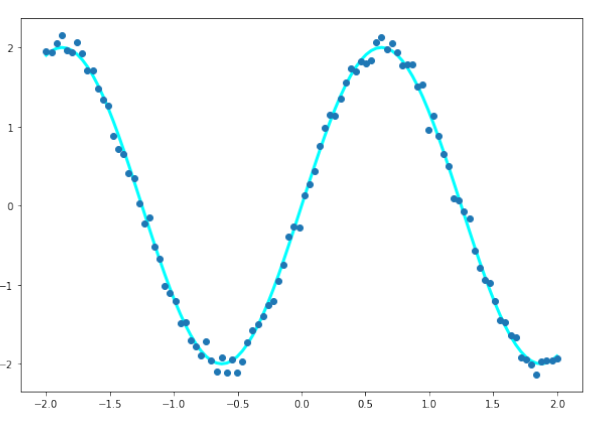
\includegraphics[width=3.4in]{a1.png}
\end{center}
\caption{Sinusoidal Dataset}
\label{fig:1}
\end{figure}
Fig \ref{fig:1} was generated by choosing
values of $t_n$, for n = 1, . . . , N, where N= 100 and spaced uniformly. Data set y was obtained by first computing the corresponding values of the function $A\sin2\pi{ft}$ and then adding a small level of random noise having a random distribution to each such point in order to obtain the corresponding value.
\begin{lstlisting}
# Data Creation
def create_data():
    t = PolynomialFeatures(degree=6).fit_transform(np.linspace(-2,2,100).reshape(100,-1))
    t[:,1:] = MinMaxScaler(feature_range=(-2,2),copy=False).fit_transform(t[:,1:])
    l = lambda t_i: 2*np.sin(0.8*np.pi*t_i)
    data = l(t[:,1])
    noise = np.random.normal(0,0.1,size=np.shape(data))
    y = data+noise
    y= y.reshape(100,1)
    return {'t':t,'y':y}
\end{lstlisting}
\section{Polynomial Curve Fitting}
To find a line that best resembles the underlying pattern of the training data shown in the graph. By using the least squares method followed by Stochastic gradient descent to corresponding estimated responses,The objective function to be minimized is
\begin{align}
Q\brak{{w}} = \sum_{i=1}^{n} Q_{i}\brak{w}
&=\sum_{i=1}^{n}\brak{\hat{y_{i}}-y_{i}}^2\\
\implies \sum_{i=1}^{n}\brak{w_{1}+w_{2}t_{i}-y_{i}}^2\\
\intertext{The Last Line in the above pseudocode for this specific problem will become,}\\
\myvec{w_{1} \\ w_{2}}:= \myvec{w_{1} \\ w_{2}} -\eta \myvec{ \frac{\partial}{\partial w_{1}}\brak{w_{1} + w_{2}t_{i} - y_{i}}^2\\ \frac{\partial}{\partial w_{2}}\brak{w_{1} + w_{2}t_{i} - y_{i}}^2}\\
= \myvec{w_{1}\\ w_{2}}-\eta \myvec{2\brak{w_{1}+w_{2}t_{i}-y_{i}}\\ 2t_{i}\brak{w_{1}+w_{2}t_{i}-y_{i}}}
%\hat{\vec{w}}\myvec{ 1 & t_{0} & t_{0}^2 & \ldots & t_{0}^{N-1} \\
%		1 & t_{1} & t_{1}^2 & \ldots & t_{1}^{N-1} \\
%		1 & t_{2} & t_{2}^2 & \ldots & t_{2}^{N-1} \\
%		\vdots & & \vdots &  & \vdots  \\
%		    1 & \ldots & \ldots & \ldots & t_{N}^{N-1} }\label{eq:2}
\end{align}
Note that in each iteration (also called update),only the gradient evaluated at a single point ${\displaystyle t_{i}}$ instead of evaluating at the set of all samples.\\
%Form the above the weight matrix we get,
%\begin{align}
%    \vec{w} = \myvec{w_{0} & w_{1} & w_{2} &  w_{3} & \ldots %& w_{N}}^T \label{eq:3}
%\end{align}
%Substituting \eqref{eq:1} and \eqref{eq:3} in Eq. \eqref{eq:2}
%we get, 
%\begin{align}
%    y= \myvec{w_{0} \\ w_{1} \\ w_{2}  \\ \ldots \\ w_{N}} \myvec{ 1 & t_{0} & t_{0}^2 & \ldots & t_{0}^{N-1} \\
%		1 & t_{1} & t_{1}^2 & \ldots & t_{1}^{N-1} \\
%		1 & t_{2} & t_{2}^2 & \ldots & t_{2}^{N-1} \\
%		\vdots & & \vdots &  & \vdots  \\
%		    1 & \ldots & \ldots & \ldots & t_{N}^{N-1} %}\label{eq:4}
%\end{align}
%
\begin{lstlisting}
def batch_gradient_descent(t,y,w,eta):
    derivative = np.sum([-(y[d]-np.dot(w.T.copy(),t[d,:]))*t[d,:].reshape(np.shape(w)) for d in range(len(t))],axis=0)
    return eta*(1/len(t))*derivative

# Update w
w_s = []
Error = []
for i in range(iterations):
    # Calculate error
    error = (1/2)*np.sum([(y[i]-np.dot(w.T,t[i,:]))**2 for i in range(len(t))])
    Error.append(error)
    w -= batch_gradient_descent(t,y,w,eta)
\end{listing}    
Code to initialize variables.\\
\begin{lstlisting}
# initialize variables
data = create_data()
t = data['t']
y = data['y']
w = np.random.normal(size=(np.shape(t)[1],1))
eta = 0.1
iterations = 10000
batch = 10
\end{lstlisting}
Code to initialize variables.\\
\begin{lstlisting}
# initialize variables
data = create_data()
t = data['t']
y = data['y']
w = np.random.normal(size=(np.shape(t)[1],1))
eta = 0.1
iterations = 10000
batch = 10
\end{lstlisting}
\begin{figure}[!h]
\begin{center}
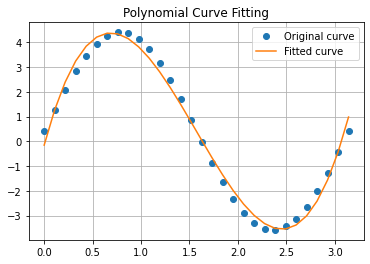
\includegraphics[width=3.4in]{a2.png}
\end{center}
\caption{Fitted Data}
\label{fig:2}
\end{figure}
Plotting the Predicted and actual plot 
\section{Observation}
\begin{itemize}
  \item Less oscillations and noisy steps taken towards the global minima of the loss function due to updating the parameters by computing the average of all the training samples rather than the value of a single sample.
\end{itemize}
Download Python codes from 
%
\begin{lstlisting}
https://github.com/ayushkesh/EE4015/tree/master/AI4
\end{lstlisting}
\end{document}
